\chapter{Architecture and Implementation}

In the previous chapter the foundation for implementing a system that does route optimization for snow plowing has been outlined. It has been shown why the NEARP has been chose as the underlying model. Further it was argued why MAs are a good approach to the problem. Then issues relating to the combination of the snow plowing problem and MAs solving the NEARP were discussed.

Now with the background for the implementation sorted out, the architecture should be addressed. The main flow of the system is illustrated in figure \ref{fig:system_flowchart}. Here we can see that the first thing to happen is that input data is converted to the NEARP format\footnote{\url{http://www.sintef.no/projectweb/top/nearp/documentation/}} for use by the MA.

\begin{wrapfigure}{o}{0.47\textwidth}
	\begin{center}
		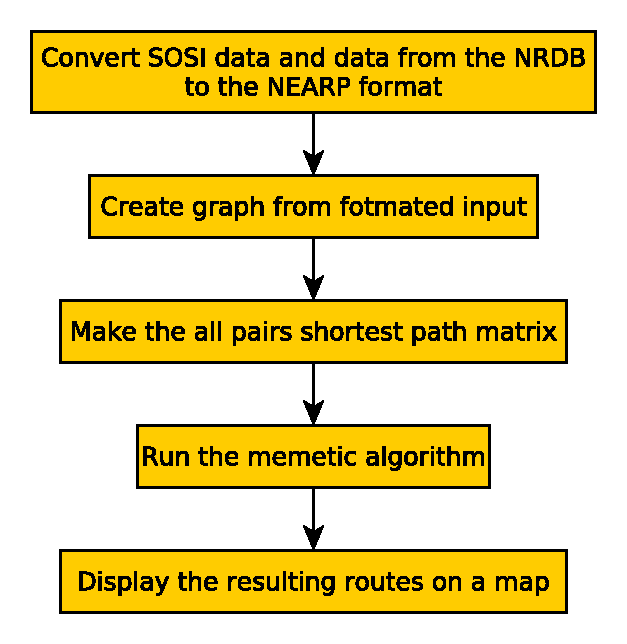
\includegraphics[width=0.46\textwidth]{figures/Architecture/Overal_system_workflow.pdf}
	\end{center}
	\caption{Overview of the systems Workflow}
	\label{fig:system_flowchart}
\end{wrapfigure}

The data comes from two main sources. The first one is the municipalitys map data, supplied in files adhering to the Norwegian SOSI-Standard for map data\footnote{\url{http://kartverket.no/en/SOSI-Standard-in-English/SOSI/SOSI-Standard-in-English/}}. Most importantly, the maps contain information about what set of roads and intersections make up each existing route. These can then be used as the the required elements of a route the MA is supposed to optimize the servicing of. The sets of roads can also be utilized for evaluating how the drivers currently drive their routes with the fitness function used by the MA. This fitness can then be used to evaluate how good the results of the MA are by comparing it to the best fitness the MA finds for the same set of roads.

Another important piece of data that the municipalitys maps contains are modifications to the infrastructure made by and maintained by the municipality. The most important example would be barriers. As shown in figure \ref{fig:environmental_factors} some of the barriers can be passed by snow plowing vehicles, while other barriers can not. The municipalitys maps detail which can and which can not be passed.

What other information about the infrastructure that is required but not contained in the municipalitys data set can be found in the NPRAs data. Their database of roads, the NRDB, contains highly detailed information about the road network. It covers physical features such as length, width, and curvature, as well as meta-information such as speed limits, placement of signs, and where pedestrian crossings are located.

The process of making an input file based on all this data is done in the following way. First the road netowrks from the municipalitys maps and the NRDB are combined into a single data set with PostGIS. This set is then converted into a graph with nodes, edges, and arcs. The intersections become nodes, and the ones that are part of a route in the municipalitys maps are labeled as required. One-way streets are converted to arcs, and other roads to edges. When working with routes for car roads, bicycle paths, pavements, and sidewalks are ignored. This is because they in most cases cannot be utilized by the vehicles operation on the car roads for passing through, and when finding routes for plowing car roads they do not have to be considered for servicing.

When making arcs and edges, the ones that are part of a route are labeled as required, just like the nodes. The arcs and edges are then assigned a traversal cost, that describes how much resources are spent passing through them without performing work on them. For car roads this was set to be the length of the road described by the arc or edge, times the speed limit on the stretch. For other kinds of underlying roads or paths the traversal cost was set to just the length.

\begin{wrapfigure}{o}{0.5\textwidth}
	\begin{center}
		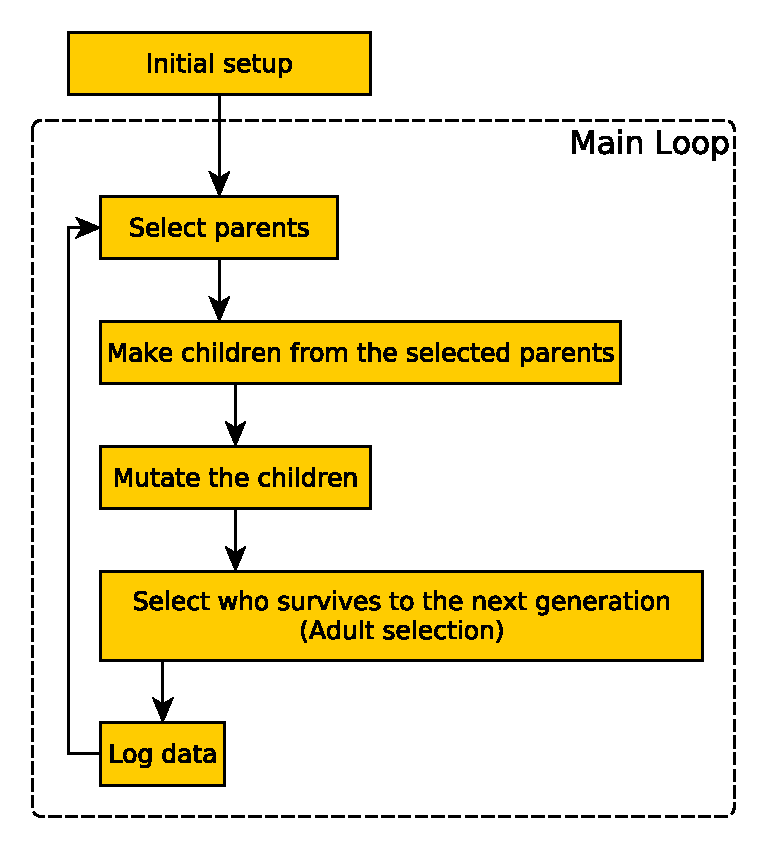
\includegraphics[width=0.5\textwidth]{figures/Architecture/MA_flowchart.pdf}
	\end{center}
	\caption{Memetic Algorithm Flowchart}
	\label{fig:ma_flowchart}
\end{wrapfigure}

After the traversal costs were determined for the arcs and edges, the required elements got their demands and servicing costs set. The demand of each element, in the case of snow plowing representing the amount of snow that each vehicle should handle the removal of, was set to be the area of the element. The servicing cost was chosen to be the speed limit of the underlying road times its area.

This process for converting to and from the NEARP format for the MA was designed in collaboration with Magnus Solheim Thrap and Christoffer Viken. We all took part in deciding how the data should be mapped to the NEARP format. Thrap found how to excract the neccessary data from the NRDB, and made a preliminary implementation relying on only those data. At a later point Viken was able to access the data in the municipalitys files, and combine the two sets. Viken then made the final implementation of the module that converts the data from the two sets to the NEARP format, and the one that takes the resulting output and draws it on a map.

Now when the implementation of how the MA takes input has been outlined, the architecture of the MA itself can be discussed. The workflow in the MA is shown in figure \ref{fig:ma_flowchart}. From the figure it can observed that the first step is generating an initial population. This population is either generated completely at random, or seeded from known routes. The seeding can be done for an instance when working with existing routes, to see whether the MA can improve on them, or if routes with better fitness can be generated faster.

\begin{figure}[thbp]
	\centerline{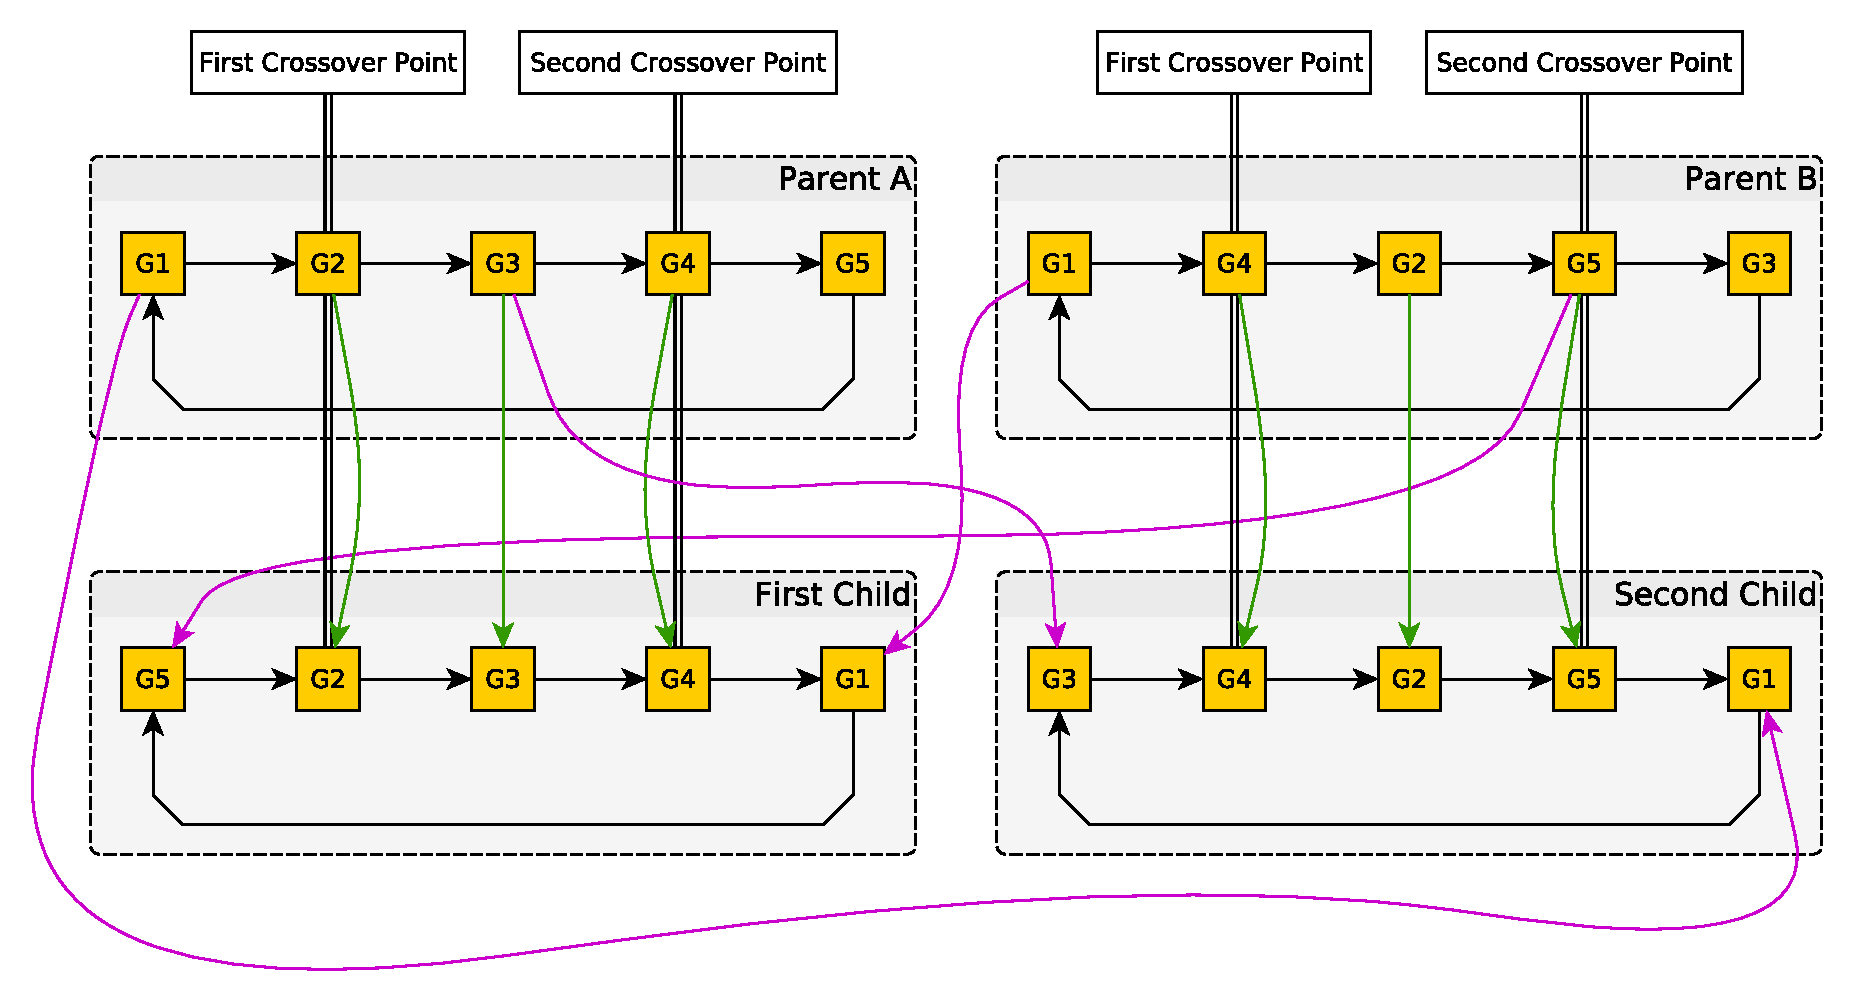
\includegraphics[width=\textwidth]{figures/Architecture/Crossover_Illustration.pdf}}
	\caption{Crossover with two parents and two crossover points}
	\label{fig:crossover_illustration}
\end{figure}

Once the initial population has been generated, the MA enters its main loop. Here it will first select which individuals get to breed in the parent selection. In the implementation, there are three possible ways of doing the parent selection. Uniform selection, fitness proportionate selection, and tournament selection. All the parent selections are implemented with replacement, but with the constraint that no pair of parents can have two equal individuals. That is, one individual can have several mates each generation, but cannot mate with itself.

If using uniform selection, the parents are selected completely at random from the adult population, ie. they have a uniform probability of being selected. The fintess proportionate selection is biased towards picking individuals with better fitness for being parents, by giving each individual a probability of being chosen that is $P(\text{selecting individual}) = \frac{\text{the fintess of the individual}}{\text{sum of fitnesses of all adult individuals}}$.

Tournament selection picks individuals for parenthood by making groups of individuals it selects from. For each parent it selects, it crteates a group of fixed size which is determined by the operator on startup, that is sorted by fitness. Then, with a chosen probability $P$ it selects the best individual. Should the best individual not be selected, it goes on to the second best, and determines whether to select it with the same probability $P$. The tournament with the individuals stacked against each other continues until a parent is selected, or all individuals other than the worst in the group have failed. In the event that all better individuals in the group fail to be selected, the worst one is selected. This gives the best individual a probability of $P$ of being selected, the worst one $(1-P)^{\text{tournament group size}-1}$, and the ones in between $(1-P)^{n} \times P$, where $n$ is the number of better individuals in the tournament group.

When the parent selection has been done, the selected pairs of parents are used for generating children with the crossover procedure, which is illustrated in figure \ref{fig:crossover_illustration}. The crossover works by first selecting two random crossover points. Then, for each parent, every element in the genome that is between these points is copied to a child genome. The rest of the cild genome that is not between the crossover points, is then filled with the remaining required elements. They are inserted in the order they appear in the other parent after the second crossover point. This process ensures the child genomes maintain their properties as circular representations of all the required elements from the graph, and that they inherit traits from both parents.

After all the children have been generated, the MA mutetes them. In the implementation this step is done by either swapping two elements in their genomes at random, or perofrming a memetic improvement of the genomes. The memetic improvement is done by swapping two and two elements in the genome, and evaluating the fitness of the outcome. This process is repeated until the swap results in an improved fintess, or all swaps have been tried.

Then, when the children have been made and mutated, the adult selection is perfomred. This is the process where one determines what individuals from the adult population and children are kept and used as adults in the next generation. There are four kinds of adult selection methods in the implementation, full replacement, elitist mixing, random mixing, and overproduction. With full replacement, there are made exactly as many children as the size of the population is at the start of each generation. In the transition, all the previous individuals are discarded, and the children become the new population.

If doing elitist mixing, the number of children can be arbitrarily chosen. When going to the next generation, the children and adults are combined into one large pool. Then the ones with the best fintesses get the slots in the new population, and all the other are discarded. Random mixing works much in the same way as elitist mixing, except that the individuals are chosen from the pool at random, instead of by fitness. The approach when using overproduction is to create more children than there are individuals at the start of the next generation. In the transition to the next generation the best children are used, and the rest of the old generation is discarded.

After the adult selection has been done, the worst individual of the new generation is removed, and the previous best is inserted in its place. Then the halting conditions for the MA are checked, and if they are met the algortihm terminates. The conditions that are checked for are whether there has been no improvements in the best individual found for a number of generations determined on startup, or whether a fixed number of generations has elapsed since the MA was started. Once it has terminated, the output can be drawn on a map.




% We have what the system should do (snow, NEARP) and how it should be done (MA, special fitness).
% Here is the architecture of the system we based upon this.
% 	Overall process
% 	External resources and output
% MA details
% 	detailed loop
% 	what we focues on in the fitness implementation
% Expected asympthotical running time
% 	parse graph |g| + flw -> |g|\^3 + MA -> generations * (number of parents * selection overhead + number of children * (generating overhead (|genome|) + fitness evaluation of each (if not split |genome/graph| else if split |genome\^2|) ) + overhead of population transitions (sorting the population (n*log n ?), selecting the next population (O(1) in our implementations), updating best knowns (O(1) also)))
% General maintainability of the implementation
% Expected future reliance of the external resources used (NRDB, sos-files)
% On to how to set up experiments for this.








% Now it is time to discuss the implementation.
% The next thing that should be discussed is the implementation.
% Once all of that is out of the way, next the implementation should be discussed.
% At this point, the implementation should be discussed.
% This brings us to how the system has been/was implemented.
% The system that sprang out of this ...
% Now that this has been discussed, 
% Now that that has been covered, it is time to look at the implementation.
% Now when we have covered that, ...
% Now that the background has been covered, one should look at the implementation
% What all of this has lead to *is the solid foundation of what comes next, the implementation*
% Now that all of that is behind us, it is time to look at the actual work behind this thesis
% All of this/that comes together in the implementation
% The implementation uses all of those things/that stuff
% The outcome of all that hard work was the implementation
% And here it is. The implementation.
% Now on to the implementation.
% The architecture that resulted
% The resulting architecture is what will be discussed next.
% All of that hard work, what for? Well here is the architecture...
% What is needed now is an explanation of the architecture of the implementation that was made 
% With the motivation and for and reasoning behind the implementation sorted out, 

% \subsection{Architectural Overview}
% Main components. NVDB and EA, written in python/java, overall workflow.

% \subsubsection{System Workflow}
% This is what happens when the system is run:

% \begin{itemize}
% 	\item The system fetches the map of Sør-Trøndelag County from NVDB.
% 	\item The user has to specify a sub-area to be processed.
% 	\item The given area is converted to a standard NEARP format (\url{http://www.sintef.no/projectweb/top/nearp/documentation/}) and written to a file.
% 	\item The user has to specify what parameters to use for the evolutionary algorithm.
% 	\item The tour calculating model produces an internal graph representation from the file with the map area, and an all pairs shortest path matrix is made.
% 	\item The evolutionary algorithm processes the graph and makes a suggested solution based on the users parameters.
% 	\item The solution is drawn on a map for readability.
% \end{itemize}

% \subsection{NVDB}

% \subsection{Internal Data Model}
% Reads graph of standard format -> Finds all pairs shortest paths using floyd warshall (mention the neat trick of including destination cost)

% \subsection{Evolutionary Algorithm}
% input: tweakable param files -> pseudocode presented as text -> mention about the memetic part

% \subsection{Heurisitc}
% What we implemented 
% -> arguing for why these are good and important things 
% -> mentioning that this doesn't solve the multi vehicle split that is oh so standard in the literature (because not relevant for our 1 car use case) 
% 	-> It could possibly be used to solve some other of trondheims probles though 
% -> mentioning what we don't take into consideration, and why one might want to look into that (ex impact of weather, slope of roads, curvature, etc)

\cleardoublepage
